\chapter{Forschungsansätze zum politischen Wandel in Europa }
Prozesse des politischen Wandels sind weltweit mit unterschiedlicher Intensität und aufgrund verschiedenartiger Impulse unter dem Einfluss unterschiedlicher Rahmenbedingungen zu beobachten. Schwerpunkte sind die Umwandlung traditionell regierter Länder zu modernen Staaten, wie insbesondere im Rahmen der westlichen Entwicklungshilfe, und aktuell die Umwälzungen in Nordafrika, sowie die Transformation vormals sozialistisch beherrschter Länder in demokratisch regierte Staaten in Osteuropa. Die Aufnahme von Staaten in die Europäische Union stellt für diese ebenfalls einen grundlegenden Wandel dar, zu dessen Beschreibung und Gestaltung allgemeine Forschungsergebnisse aus den verschiedenen Prozessen des politischen Wandels herangezogen werden können. Die Forschungsrichtung der Europäisierungsforschung und hier insbesondere das Konzept der Konditionalität ist der vorherrschende Ansatz zur Erklärung verschiedenster Prozesse, welche die EU als supranationale Organisation entfaltet. Die Europäisierungsforschung wird in diesem Kapitel als zentraler Ansatz ausführlich dargestellt, insbesondere die in ihrem Umfeld entwickelte Konditionalitätsforschung. Diese Forschungsrichtung ist von besonderer Bedeutung für die vorliegende Arbeit, da die Verwaltungsmodernisierung ein wesentliches Element der EU-Bedingungen für die Aufnahme der Westbalkanstaaten ist. Im Folgenden werden diese Forschungsrichtungen aus der Transitionsforschung hergeleitet mit den konkreten Fragestellungen der Europäisierungsforschung und der Konditionalitätsforschung. 
\section{Transitionsforschung}
Die Transitionsforschung, die sich traditionell mit Entwicklungsländern beschäftigte, erfuhr durch die politische Wende in Osteuropa eine neue Ausrichtung. Nach dem Systemwechsel in den Ländern Mittel- und Osteuropas war die wissenschaftliche Aufarbeitung der Geschehnisse zunächst von wirtschaftswissenschaftlichen Konzeptionen beherrscht, die sich vor allem mit dem Wechsel der Wirtschaftsweise von zentraler Planwirtschaft zu Marktwirtschaft befassten. Die auch stattfindenden politischen Transformationsprozesse wurden in der Folge ebenfalls nach und nach mit Erklärungsmodellen begleitet. Es entstanden Staatenanalysen und Untersuchungen spezifischer Systembereiche mit ökonomischem, demokratietheoretischem oder soziologischem Schwerpunkt (vgl. \cite{huszak}: 54ff).\par
König definiert den Prozess der Transition in den neu entstandenen Ländern Osteuropas eher als einen der Transformation. „It is evident that in the transition from command to market economy and from totalitarian state to a pluralist state, creating multiparty democracy is not only a transition in itself but rather a long process of transformation. It requires essential reforms in the basic functions and institutions of the state” (König 1992, zit. nach \cite{jenei}). \par
Der Einfluss der EU als einer der wesentlichen Geber kam zunehmend in den Blick als externer Akteur der Transformation. Von Beyme konstatiert in diesem Zusammenhang, dass der „internationale Einfluss der etablierten Demokratien auf die neuen Systeme (…) eine neue Dimension in der Weltgeschichte“ darstellt (\cite{beyme}: 158). Whitehead geht von drei Formen der Demokratisierung aus, erstens der auferlegten Demokratisierung, zweitens Demokratisierung durch Dekolonisierung und drittens Demokratisierung durch Konvergenz (vgl. \cite{whitehead}). Pridham entwickelt ein Konzept der interaktiven Prozesse zwischen externen (vor allem internationalen Organisationen) und innerstaatlichen Akteuren (vgl. \cite{pridham91,pridham95,pridham08}), während das Konzept der Diffusion bzw. einer Art „Schneeballeffekt“ bei der Demokratisierung von Huntington stammt (vgl. \cite{hunting}). Eine Aufarbeitung des Systemwandels in Osteuropa unter Betrachtung externer Faktoren findet statt; diese werden allerdings noch nicht in einem ausreichenden Maße in theoretische Erklärungszusammenhänge eingebunden: „…even though the influence of international factors has been widely acknowledged, these still have not been fully integrated into theoretical frameworks aiming to explain the dynamics or failure of post communist transitions“ (\cite{dimpri}: 93).\par
Im Rahmen der Transitionsforschung wird der Erkenntnis, dass der Beitritt zur EU spezifische Transformationsergebnisse zeitigt, zunehmend Raum gegeben. Die Forschung zum Institutionenwandel zentralstaatlicher Administration in nachkommunistischen Ländern im Rahmen der Transformations- und Integrationsforschung ist dagegen noch eher unterentwickelt. Nur selten wird auf die Entwicklung der Ministerialbürokratien und Regierungen in einem engeren Sinne Bezug genommen. Insbesondere Probleme mit der administrativen Kapazität der neuen Mitgliedsländer werden, so Lippert und Umbach, lediglich auf allgemeine Weise abgehandelt. “Therefore, the cross-country research on the administrative developments under the pressure of Europeanisation is particularly relevant” (\cite{lipumb05}: 17). Auch Luchterhand konstatiert schon 2001 im Vorwort seiner Analyse zu Verwaltung und Verwaltungsrecht im Erneuerungsprozess Osteuropas: „Dass die tatsächliche Erfüllung der Beitrittsvoraussetzungen – unterhalb einer demokratischen und menschenrechtskonformen Verfassung – nicht nur von einem EU-kompatiblen Wirtschaftssystem abhängt, sondern kaum weniger von einer leistungsstarken und rechtsstaatlich fundierten öffentlichen Verwaltung, hat man daneben weithin kaum zur Kenntnis genommen“ (\cite{lucht}: 6).\par
Die Transitionsforschung mit ihrer Untersuchung des politischen Wandels ist für die vorliegende Arbeit besonders fruchtbar. Im Zuge der EU-Erweiterung kam auch die EU als externer Akteur mit Einfluss auf Beitrittsländer in den Blick der Transitionsforschung. Die Betrachtung des Institutionenwandels als erklärtem Ziel dieser Forschungsrichtung bietet sich somit auch für die Betrachtung der Verwaltungsentwicklung an. 
\section{Neo-Institutionalismus als Ansatz zur Erklärung des Wandels}
Der Neo-Institutionalismus, der von einer zentralen Bedeutung der Institutionen für soziales Handeln ausgeht, kann als Gegenbewegung zu dem in den USA seit den 1960er Jahren dominanten „Behaviouralismus“ betrachtet werden. Dieser versuchte politische Phänomene vor allem über individuelle Einstellungen und individuelles Verhalten zu erklären. Ausgangspunkt der Kritik an einem rein verhaltenswissenschaftlichen Erklärungskonzept war die fehlende Erfassung der wachsenden Bedeutung von Institutionen. Der Zusammenbruch der Staaten in Ost- und Mitteleuropa und die damit einsetzende Erforschung der Transformationsprozesse brachte die Institutionen erneut in den Blick. Die zunächst vorherrschende Einschätzung, dass in diesen Ländern im Wesentlichen eine „nachholende Modernisierung“ stattfindet, wurde angesichts wirtschaftlicher Probleme und ethnischer Auseinandersetzungen zunehmend fragwürdig. Die Sichtweise verschob sich zunehmend hin zur Annahme, dass die Wandlungsprozesse nicht in logischer Folge ablaufen, sondern dass man von Prozessen ausgehen muss, die geprägt sind von Verteilungskämpfen und traditionellen institutionellen Einflüssen. So „finden sich in den Gesellschaften Ost- und Mitteleuropas zahlreiche so genannte institutionelle Hinterlassenschaften (institutional legacies), d.h. Routinen, Regeln und soziale Bindungen, die den Verlauf der Transformation maßgeblich beeinflussen“ (\cite{schulze}: 5). Es wird also nach der Veränderung des institutionellen Gefüges durch Anpassungsprozesse unterschiedlichster Art und Geschwindigkeit gefragt. \par
Im „neuen“ Institutionalismus in der Politikwissenschaft, der seit den 1970er Jahren verstärkt zum Einsatz kommt, unterscheidet man im Wesentlichen drei Varianten.\par
Erstens gibt es eine stark vom Rational-Choice-Ansatz bestimmte Richtung, die sich mit der Wirkung politischer Institutionen in den verfassungsmäßigen Entscheidungsgremien befasst.
In Rational-Choice-Ansätzen ist das politisch-soziale System Untersuchungsgegenstand. Grundlage für die Analyse ist das Konzept des methodologischen Individualismus, wonach Entscheidungen immer nur von weitgehend rational handelnden Individuen getroffen werden können und somit Handlungen von Kollektiven (z.B. Behörden) eine Anhäufung von Einzelfallentscheidungen seien. Dabei werden strukturelle Faktoren weitgehend ausgeblendet bei vorwiegender Berücksichtigung der angenommenen Interessen der beteiligten Akteure. Putnam entwickelt für den Blick auf die europäische Integration ein Zwei-Ebenen-Modell. Er geht davon aus, dass bei Verhandlungen über internationale Kooperationen gesellschaftliche Akteure auf nationaler Ebene Druck auf die Regierung ausüben, um ihre Ziele zu realisieren. Gleichzeitig werden von den nationalen Regierungen die Verhandlungen auf internationaler Ebene genutzt, um den Erwartungen der einheimischen Akteure nachzukommen bzw. zu entkommen (vgl. \cite{putnam}). Kritik an den akteursorientierten Ansätzen zielt vor allem auf die mangelnde Berücksichtigung struktureller und institutioneller Rahmenbedingungen ab.\par
Zweitens gibt es eine kulturalistisch-konstruktivistische Variante, die sich vom Rational-Choice-Modell abgrenzt. Hierfür steht der Ansatz von March und Olsen. Diese definieren Institutionen als ein Gefüge aus Regeln und Verhaltensroutinen, die durch soziale Werte und Normen bedingt sind und so die Akteursreaktionen beeinflussen. Es können daher kaum identisch ausgeprägte Institutionen bei unterschiedlichen kulturellen und sozialen Rahmenbedingungen entstehen (vgl. \cite{marols}: 17).\par
Drittens gibt es die vermittelnde Variante des sogenannten historischen Institutionalismus. (\cite{haltay, steinmo}). Die Wirkung von Institutionen wird historisch sowie national und sektoral vergleichend untersucht. Der historisch-soziologische Ansatz entspringt der vergleichenden Regierungslehre und stellt den Staat als zentralen Akteur mit seinen Machtpotenzialen in den Mittelpunkt.\par
Im Zentrum der Untersuchungen im Rahmen des Neo-Institutionalismus stehen die Beweggründe für institutionelle Änderungen und die Frage, wie die neuen Spielregeln nach Überwindung der alten Regeln und Handlungsmuster verfestigt und angenommen werden. Vor allem die Mechanismen des Wandels sind im Blick sowie der Einfluss des veränderten Umfelds auf die Politikgestaltung (vgl. \cite{huszak}).\par
Kennzeichnend für die aktuellen Forschungen nach den neo-institutionalistischen Konzepten ist die Konzentration auf die Bedeutung der Institutionen bei der Betrachtung gesellschaftlichen Wandels. Dies geschieht insbesondere in Abgrenzung zu verhaltenswissenschaftlichen Erklärungsansätzen, die in den Sozialwissenschaften in den USA seit den 1960er Jahren vorherrschend waren. Die Europäisierungsforschung kann als eine Weiterentwicklung der neo-institutionellen Theorien gesehen werden. \par
Auf Basis der bisher dargestellten Ansätze zum politischen Wandel wird zunächst die Europäisierungsforschung näher beleuchtet; diese stellt eine weitere Konkretisierung der Transitionsforschung im Zusammenhang mit der EU-Erweiterung dar. In einem weiteren Schritt wird auf eine Unterkategorie der Europäisierungsforschung, die Konditionalitätsforschung, eingegangen. Forschungen zur Konditionalität haben insbesondere in Bezug auf die politischen Kriterien im Erweiterungsprozess Relevanz. Die Verwaltungsentwicklung in den Beitrittsländern wird von der EU nach politischen Kriterien betrachtet. 
\section{Europäisierungsforschung}
Die Rolle der EG/EU im Zusammenhang mit Demokratisierung war im Prinzip vor 1989 nicht im Blick der Forschung und auch anlässlich der Süderweiterung (überraschenderweise) nicht beleuchtet worden (vgl. Kneuer 2007). Bezogen auf Mittel- und Osteuropa beschäftigte sich die Europaforschung vor allem mit den technischen Aspekten der Assoziierung (Europaabkommen) im Rahmen des Heranführungs- und Beitrittsprozesses (\cite{lipbec, lipsch}). Weiterhin wurden die sich entwickelnden Beziehungen zwischen der EU und den Beitrittsländern thematisiert (\cite{mayhew, torre}). Die klassische Integrationsforschung beleuchtete vor allem, ob und wie die Mitgliedstaaten auf die Entwicklung supranationaler Institutionen und Politiken einwirkten. Ein Perspektivwechsel seit Mitte der 1990er Jahre führte zur zunehmenden Beschäftigung mit der Frage nach dem Einfluss der EU und den Effekten auf nationale Systeme (vgl. \cite{kneuer09}: 21). Damit war der Paradigmenwechsel vollzogen und die nun Europäisierungsforschung genannte Betrachtungsweise basierte auf der These, dass die EU unterschiedliche Effekte in den Mitgliedstaaten hervorrufen kann. Die einsetzende Theoriebildung versuchte den Einfluss und die Wirkung der EU auf die Mitgliedstaaten und die dort ablaufenden Prozesse, Politikinhalte, Einstellungen und Normen zu beschreiben (\cite{boerzel, boeris00, radaelli00, kohler, fearad03}). Es wurde der Frage nachgegangen, ob die EU zu policy-Veränderungen führt, zur Transformation von Institutionen, oder sogar zu Identitätsveränderungen (\cite{meny, knilen, fearad03, boeris07}). \par


Im Allgemeinen wird unter Europäisierung das Zusammenwirken der folgenden drei Zusammenhänge verstanden: 
\begin{itemize} \itemsep1pt \parskip0pt \parsep0pt
\item Die Herausbildung und Entwicklung spezifischer Strukturen von „Governance" auf europäischer Ebene (vgl. \cite{risseetal}: 3, \cite{radpas}: 36).
\item Europäisierung als „top-down“-Prozess, der durch Institutionen und Entscheidungen auf der Ebene der EU die nationalen policies und Institutionen formt (vgl. \cite{herit}).
\item Ein Prozess mit folgenden Schritten: a) Konstruktion, b) Diffusion und c) Institutionalisierung von Normen, Glaubenssätzen und informellen Regeln, Abläufen, policy-Paradigmen, Stilen und „der Art wie Dinge getan werden“. Diese sind zunächst durch den EU-policy-Prozess definiert, werden dann auf die nationale Ebene übertragen und in die öffentlichen Debatten, politischen Vorgaben und Institutionen übernommen. Diese letzte Beschreibung basiert auf der Annahme der Europäisierung als Institutionalisierung und interaktivem Prozess, der über einen ein-direktionalen Mechanismus als Reaktion auf Europa und auch über das Konzept des „impact“ oder Einflusses der EU auf nationale Systeme hinausgeht. Damit ist keine vertikale Anpassung gemeint, sondern ein Sozialisierungsprozess im umfassenden Sinne (vgl. \cite{fearad03, olsen}).
\end{itemize}
Der letztgenannte Ansatz betrachtet unter verschiedenen Blickwinkeln und in einer diskursiven Herangehensweise, wie nationale Veränderungen geschehen. Zwar kann man mit definierten Kriterien den Grad der Europäisierung messen oder zumindest beschreiben, allerdings ist ein besonderes Problem immer die Abgrenzung von Anpassung und Transformation (vgl. \cite{radpas}: 40).\par
Die klassischen Probleme der Forschung zur Europäisierung sind a) Voreingenommenheit bei der Beurteilung des Einflusses der EU auf die nationalen policies und die Politik und b) die Annahme, dass es sich bei nationalen Veränderungen, die den Brüsseler Vorschlägen ähnlich sind, um Europäisierung handelt (vgl. \cite{radpas}: 40). Oder wie Goetz warnt: „Europeanization can very easily become a cause in the search of an effect (at the domestic level)” (\cite{goetz01a}: 211). Noch kritischer wird von Mair angemerkt: „Europeanization and globalization are becoming catch-all, default explananda for almost everything that cannot otherwise be explained at the domestic level” (\cite{mair}: 339).\par
Die Konzepte der Europäisierung wurden zunächst fast ausschließlich auf Mitglieder der EU angewandt. Erst seit der letzten Erweiterungswelle gibt es Studien, die sich im Rahmen der Europäisierungsforschung auch mit Regionen außerhalb der Grenzen der EU beschäftigen (\cite{lipumwes, grab03, papadi, lavenex, schsed05b, schsed05c}). Die aktuellen Ansätze der Europäisierungsforschung sind für empirische Studien vor allem in drei Richtungen nutzbar gemacht worden: Europäisierung als Policy-Veränderung, Europäisierung als Institutionenveränderung sowie Europäisierung und EU-Erweiterung. Diese drei Stränge der Europäisierungsforschung werden im Folgenden kurz dargestellt.
\subsection{Europäisierung als Policy-Veränderung}
Eine Reihe von empirischen Studien wurde zur Europäisierung der politischen Institutionen und Entscheidungsprozesse einzelner Staaten oder als Ländervergleiche durchgeführt. Vor allem Frankreich, Deutschland und Großbritannien dienten dabei als Untersuchungsländer. Weiterhin gibt es Untersuchungen zu einzelnen policy-Feldern. Hier wird oft nach der nationalen Umsetzung der EU-Vorgaben in den Mitgliedstaaten gefragt. Studien in dieser Kategorie beschäftigen sich bislang vor allem mit Umweltpolitik, Sozial- oder Regionalpolitik, seltener mit Landwirtschafts-, Gesundheits-, Wettbewerbs- oder Kulturpolitik. Die Themen Außen- und Sicherheitspolitik sowie Justiz- und Innenpolitik waren bislang selten im Forschungsinteresse, mit Ausnahmen bei der Immigrations- und Asylpolitik (vgl. \cite{bulmer07}: 57). Die vorgelegten Studien zeigen, dass der Einfluss der EU im Bereich der Umweltpolitik und der Sozialpolitik zu höheren Standards in den Mitgliedsländern geführt hat, wobei die südlichen Mitgliedstaaten stärker von Veränderung betroffen waren. Auch wurden neue Instrumente der Politikgestaltung übernommen, die z.B. auf einer stärkeren Einbeziehung von verschiedenen sozialen Gruppen basieren oder auf politikfeldübergreifender Kooperation. In Bereichen, in denen die EU großen Einfluss hat und Eingriffe vornehmen kann, ist es dennoch nicht zu einem einheitlichen Politikstil gekommen (vgl. \cite{boeris07}: 486).
\subsection{Europäisierung als Institutionenveränderung }
Studien in diesem Bereich haben sich mit Fragen beschäftigt, inwieweit europäische Prozesse sich auf die Beziehungen zwischen Regierungen, nationalen Bürokratien und administrativen Prozessen, Regulierungsstrategien, Justizstrukturen oder die Beziehungen zwischen Legislative und Exekutive auswirken. Diese Arbeiten kommen zu keinem eindeutigen Ergebnis. Manche Untersuchungen fanden heraus, dass nationale Institutionen dem europäischen Einfluss im Wesentlichen standgehalten haben, während andere Studien davon ausgehen, dass die EU die nationalen Systeme föderalisiert oder pluralisiert habe. Börzel und Risse sehen in diesen Ergebnissen die Kontroverse gespiegelt, ob die EU-Integration den Staat stärkt, schwächt oder transformiert. Für nationale Verwaltungen konstatieren sie, dass diese die Anforderungen der EU erfüllt haben, aber die konkrete Umsetzung unterschiedlich ausfällt und maßgeblich von den schon existierenden Institutionen abhängt. „National administrations have responded to the ‚demands of EU membership’ but institutional adaptation differs significantly and is mediated by pre-existing institutions“ (\cite{boeris07}: 487).
\subsection{Europäisierung und EU-Erweiterung }
Die EU-Erweiterung nach Osteuropa bot eine gute Möglichkeit, die Hypothesen der Europäisierungsforschung zu testen. Die Länder Ost- und Mitteleuropas, insbesondere die post-kommunistischen Länder, hatten eine andere historische Einbindung als westeuropäische Demokratien und sie hatten wenig Möglichkeit, selbst Einfluss auf die EU-Politik auszuüben. Diese Länder mussten den Acquis communautaire übernehmen und standen damit unter einem erheblichen Anpassungsdruck. Damit verbunden war die Vermutung, dass sie die EU-Modelle stärker internalisieren aufgrund der Schnelligkeit, mit der sie EU-Vorgaben übernehmen mussten angesichts des großen Umfangs der zu übernehmenden EU-Agenda und dank der größeren Offenheit für EU-Modelle im Rahmen des post-kommunistischen Transformationsprozesses (vgl. \cite{grab03}). Doch die Studien zeichnen kein eindeutiges Bild. Die meisten Forscher stimmen darin überein, dass die EU-Erweiterung den Hauptstimulus darstellte und die Übernahme des Acquis communautaire die Aufnahmebedingung war. Dies bedeutete auch, dass Europäisierung in diesem Zusammenhang eher ein „top-down"-Prozess und eine „Einbahnstraße“ war. Zwar zeigte sich, dass die wesentlichen Verwaltungseinheiten gestärkt wurden, die Entwicklung eines nicht-politisierten civil service begünstigt wurde und ein gewisser Grad an Dezentralisierung erreicht wurde, zumindest im Gegensatz zur kommunistischen Zeit. Dennoch variieren die Auswirkungen auf Institutionen und Politik erheblich.\par
Zusammenfassend kann gesagt werden, dass die Europäisierungsforschung im Rahmen der Transformationsforschung entstanden ist. Zunächst wurde vor allem der Einfluss der EU auf nationale Politik und Institutionen in den Mitgliedsländern untersucht. In der praktischen Anwendung auf unterschiedliche Politikfelder stellte sich heraus, dass vor allem im Bereich der Umwelt- und Sozialpolitik durch Anforderungen der EU insgesamt höhere Standards zur Durchsetzung kamen.
\par
In der vergleichenden Betrachtung zur institutionellen Veränderung durch EU-Politik zeichnen entsprechende Studien kein eindeutiges Bild. In einigen Fällen wird ein Standhalten der Institutionen gegenüber EU-Einflüssen konstatiert, während andere Untersuchungen von einer Pluralisierung der nationalen Systeme ausgehen.\par
In Bezug auf die EU-Erweiterung kommt die Europäisierungsforschung ebenfalls zu unterschiedlichen Einschätzungen. Allerdings geht die Mehrheit der Untersuchungen von einem „top-down“-Prozess aus, der mit der Übernahme des Acquis communautaire als Beitrittsbedingung verbunden ist. Nach diesen Studien wurden europäische Standards nur vordergründig übernommen, um den Anforderungen für eine EU-Mitgliedschaft zu genügen. Eine wesentliche Institutionenveränderung hätte nach dieser Sichtweise nicht stattgefunden. Dies vor allem, weil unter Zeitdruck ein umfassendes soziales Lernen als Voraussetzung für Veränderungen der nationalen Institutionen nicht stattgefunden hat.
\section{Konditionalität als Konzept}
Das Konzept der politischen Konditionalität kommt aus der Entwicklungszusammenarbeit als ein Instrument bei der Durchsetzung von Reformen, die explizit oder implizit auf Demokratisierung abzielen. Dabei werden generell positive und negative Konditionalität unterschieden. Positive Konditionalität macht die Mittelvergabe von der Implementierung von Reformmaßnahmen abhängig, während negative Konditionalität die Kürzung oder Einstellung der Unterstützungsleistungen bedeutet, wenn die Empfängerseite vereinbarte Auflagen nicht eingehalten hat (vgl. \cite{schmitz09}: 127). Bis in die 1990er Jahre waren Zuwendungen der internationalen Finanzinstitutionen meist mit Strukturanpassungsmaßnahmen verbunden, die von den Empfängerländern durchzuführen waren. Untersuchungen zur Wirksamkeit solcher Programme kamen generell zu dem Ergebnis, dass die Wirksamkeit der ökonomischen Konditionalität der Strukturanpassungsprogramme oft nicht nachweisbar ist oder bestehende Probleme noch verschärft wurden (\cite{killick, morrissey}). 
\par
Eine andere Richtung schlagen die Konzepte „policy transfer“ und „lessons learning“ vor. Diese entstammen dem Forschungsfeld der Vergleichenden Politikwissenschaft, das vor allem in den 1990er Jahren neue Impulse entwickelte. Gefragt wird hier, wie nationale Politik durch das Lernen von erfolgreichen Beispielen anderer Länder verbessert werden kann. Der Bertelsmann-Index und der Governance-Index der Weltbank stehen in dieser Tradition. Die neue Denkrichtung geht von einer „demokratisierten“ Konditionalität aus, die als wechselseitiger Prozess verstanden wird, in dessen Verlauf sich Geber und Empfänger auf gemeinsame Ziele verständigen unter Einbezug von Dialog und Monitoring.
\subsection{Konditionalitätsforschung im Rahmen der Europäisierungsforschung }
Der zunehmende Gebrauch der Konditionalität seitens der EU in den späten 1990er und frühen 2000er Jahren ging einher mit einer Expansion der Forschung zum Einfluss der Konditionalität auf unterschiedliche Länder, Politikfelder und institutionelle Gegebenheiten (\cite{grab99, grab01, grab03, schsed04, schsed05b, schsed05c, vachudova01, vachudova05}). Es sind einige vergleichende Studien entstanden zu den Demokratisierungseffekten der EU. Diese Arbeiten kommen zu einer Reihe von übereinstimmenden Erkenntnissen hinsichtlich der Effektivität der EU als Demokratie-Förderer. Es wird davon ausgegangen, dass die Anwendung von Konditionalität wesentliche Erfolgsvoraussetzung ist. Dabei ist zunächst politische Konditionalität zu nennen (\cite{kelley, kubicek, pridham05, schetal, vachudova05, youngs}). Die als wahrscheinlich angenommene Aufnahme in die EU bei erfolgreichen demokratischen Reformen wird als das effektivste Element der EU-Strategien eingeschätzt. Weiterhin stimmen die Studien darin überein, dass außerhalb von Europa, d.h. ohne Mitgliedsperspektive, die politische Konditionalität mit ihrer Demokratieförderung weniger erfolgreich ist. Grundsätzlich kommen die Untersuchungen zu dem Ergebnis, dass sogar in einer Situation, wo die Mitgliedsperspektive sehr glaubhaft ist, weitere Faktoren hinzukommen müssen. Förderliche politische Umstände in den Zielländern sind dabei wesentlich, um einen positiven Demokratisierungseffekt zu erreichen (vgl. \cite{schsch07}: 273).\par
Inzwischen liegen auch einige empirische Untersuchungen zu den Auswirkungen des EU-Beitritts in den mittel- und osteuropäischen Staaten vor (\cite{dimit02, grab05, kneuer07, linden, schsed05a}). Diese Studien gehen von einer generell erfolgreichen Wirkung der EU-Konditionalität aus, da die Reformen in den entsprechenden Ländern umgesetzt wurden oder Regierungen, die von der EU kritisiert wurden, abgewählt wurden (vgl. \cite{brusis09}: 196).\par

Einen Überblick zu den Ansätzen zur Erforschung des Europäischen Integrationsprozesses im Hinblick auf institutionelle Strukturen der Mitgliedstaaten liefert folgendes Schema:
\begin{figure}[H]
\setlength\belowcaptionskip{10pt}
 \centering
\caption{ Überblick über die Forschung zu Europäisierung und Konditionalisierung}
 
  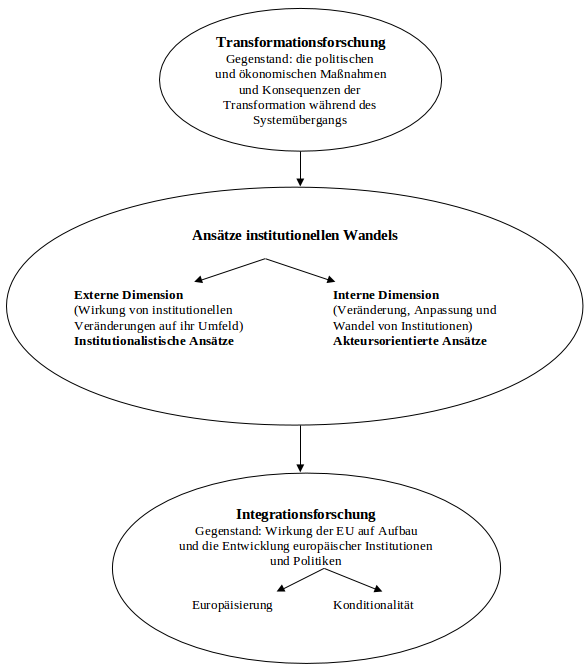
\includegraphics[width=5in]{Material/ForschungZuEuropUndKondi_ohneRand}\\

Quelle: in Anlehnung an \cite{huszak}: 75.
  \end{figure}
Erkennbar ist aus diesem Schema die Einbettung der Europäisierungs- und Konditionalitätsforschung in die übergeordneten theoretischen Konzepte Integrationsforschung, Forschung zu institutionellem Wandel und Transitionsforschung.\par
Moravcsik und Vachudova gehen von einer asymmetrischen Interdependenz zwischen Beitrittskandidat und der EU aus. Bei positiv verlaufender Konditionalität schätzen die Kandidatenländer die politischen Kosten der Anpassung ihrer nationalen Politiken niedriger ein als einen möglichen Ausschluss aus der EU und die damit verbundenen Nachteile (vgl. \cite{morvac}: 44).
\par
Schimmelfennig und Sedelmeier schlagen ein „external incentives“-Modell vor, das den Erfolg der EU-Konditionalität anhand von vier Faktoren beschreibt. Diese Faktoren führen dazu, dass nationale Regierungen EU-Regeln übernehmen, wenn die Vorteile größer sind als die Kosten der Anpassung. Die vier Faktoren sind “the determinancy of conditions, the size and speed of rewards, the credibility of threats and promises and size of adaption costs” (\cite{schsed05b}: 12). Angewandt auf die neuen EU-Mitgliedsländer kommen die Autoren zu dem Schluss, dass das „external incentives“-Modell von dem Typ der Konditionalität abhängt, wobei die Acquis-Konditionalität besser abschneidet als die politische Konditionalität (vgl. \cite{schsed05c}: 212). Die empirische Überprüfung führt zu dem Schluss, dass die Glaubwürdigkeit der Belohnung und die Höhe der politischen Anpassungskosten ausschlaggebend waren bei der Entscheidung der Anpassung an EU-Konzepte. Hinsichtlich der Glaubwürdigkeit erhöhte die Eröffnung von Verhandlungen die Wahrscheinlichkeit von nationalen Anpassungen, da sich damit in den Augen der Kandidatenländer der Wille der EU zeigte, die Verhandlungen auch zu einem Abschluss zu bringen (vgl. \cite{schsed05c}: 215). Weiterhin nimmt die Gefahr des Ausschlusses von der EU-Mitgliedschaft ab, je weiter der Assoziierungsprozess fortschreitet (vgl. \cite{dimit05}). Allerdings zeigte sich auch, dass hohe Anpassungskosten, die die Sicherheit oder Integrität des Staates oder das Überleben der Regierung gefährdeten, eine starke Behinderung darstellten, sogar bei glaubwürdigen Anreizen der EU. Nur im allerletzten Stadium der Verhandlungen („endgame“) haben die Staaten die Anpassungsleistungen vollzogen, sogar bei kurzfristigen hohen politischen Anpassungskosten im eigenen Land (vgl. \cite{schetal}: 921).\par

Huszka merkt in Bezug auf die Anwendung dieses „external incentives”-Modells auf den Balkan an: „However, while this ‘external incentive model’ according to which external rewards help elites to overcome domestic costs worked effectively in Central and Eastern Europe, its application to the Western Balkans is more problematic” (\cite{huszka}: 10). Hinzu kommt, dass die Mitgliedschaft für die in der vorliegenden Arbeit betrachteten Balkanstaaten noch stark in der Zukunft liegt. Daher sind die Belohnungen, die aktuell möglich sind, eher beschränkt.\par

Brusis konstatiert, dass demokratische Reformen verschiedene Ursachen haben und er geht davon aus, dass die Konditionalität der EU einen wesentlichen Einfluss hat, gibt aber auch zu bedenken: „Von der EU oder anderen externen Demokratisierungsakteuren gestellte Anforderungen sind aber weder a priori notwendige, noch hinreichende Bedingungen für innerstaatlichen Wandel“ (\cite{brusis05}: 298).

\subsection{Öffentliche Verwaltung und politische Konditionalität}

Die Notwendigkeit einer stabilen, effektiven und transparenten Verwaltung ist im Hinblick auf die Fähigkeit zur Übernahme des Acquis communautaire wichtig und wird in den Handreichungen der EU zur Übernahme des Acquis folgendermaßen formuliert: “A candidate country preparing for accession to the EU must bring its institutions, management capacity and administrative and judicial systems up to Union standards with a view to implementing the acquis effectively… At the general level, this requires a well-functioning and stable public administration built on an efficient and impartial civil service, and an independent and efficient judicial system” (\cite{eurcom05}: 7).\par
Die Existenz einer gut funktionierenden und stabilen öffentlichen Verwaltung ist eines der wesentlichen Kriterien innerhalb der EU-Konditionalität. Allerdings ist die öffentliche Verwaltung kein Kapitel des Acquis und unterliegt damit nicht der direkten Überprüfung anhand eines Kriterienkataloges. Die EU hat gemeinsame grundrechts- und allgemein rechtsstaatsbezogene Normen aufgestellt. Doch gibt es keine konkreten Vorgaben, wie demokratische Institutionen (Parlament, Regierung, Gerichte, Verwaltungsaufbau) organisiert sein sollen. Und in dieser Hinsicht existieren keine konkreten benchmarks, an denen sich die Beitrittsländer orientieren und deren Erfüllung man untersuchen könnte (vgl. \cite{brusis09}: 196). Von der EU wird das Thema Verwaltungsreform unter „politische Bedingungen“ behandelt und diese „politischen Kriterien“ nehmen einen festen Raum ein in den jährlichen Fortschrittsberichten der EU zu den Beitrittskandidaten.\par
Die Konditionalitätsforschung geht also von einem starken Zugzwang aus, in den die Kandidatenländer geraten, der dazu führt, dass sie die Anforderungen der EU zum Umbau ihrer nationalen Strukturen erfüllen. Dies wird deutlich im Rahmen der geforderten Übernahme des Acquis mit konkreten Kapiteln, die im nationalen Rahmen umzusetzen sind. Im Zusammenhang mit der Verwaltungsmodernisierung ist dies nicht so eindeutig nachvollziehbar, da es sich nicht um ein Kapitel des Erweiterungsacquis handelt.\par
Kennzeichnend für die Konditionalitätsforschung ist also die Konzentration auf die Frage, was die Veränderungen insbesondere in den Beitrittskandidaten befördert. Zentraler Gesichtspunkt sind dabei die Bedingungen der EU, die einem Beitritt vorausgehen, d.h. die Konditionalität. Im Kontext der vorliegenden Arbeit geht es hierbei insbesondere um die politische Konditionalität, unter die das Thema Verwaltungsmodernisierung fällt, ist kein Kapitel des Acquis und entfaltet daher vergleichsweise geringere Konditionalität. Dennoch wird die Struktur der Verwaltung und ihre Modernisierung bei den politischen Kriterien abgehandelt, wie z.B. in den jährlichen Fortschrittsberichten deutlich wird.\par
Insofern ist die Konditionalitätsforschung auch auf das Thema Verwaltungsmodernisierung in den Beitrittsländern anwendbar und kann wertvolle Hinweise liefern. \par
Im nächsten Abschnitt der Untersuchung werden deshalb die praktischen Aspekte der EU-Erweiterung, jeweils mit Rückbindung an das Thema Verwaltungsentwicklung und Verwaltungsmodernisierung, überblicksartig dargestellt. Es wird im weiteren Verlauf der Arbeit zu prüfen sein, welchen Stellenwert Verwaltungsmodernisierung für die EU im Zuge der Erweiterungsstrategie hat und wie Verwaltungsmodernisierung in der Erweiterungspolitik vorkommt.
